\begin{problem}{Mostrando grafos}{Standard input}{Standard output}{1 second}{}

% Original idea         
% Problem statement     
% Testset               

En la clase de algoritmos y estructuras de datos, el profesor estaba explicando el tema de árboles y Gerardo (uno de sus estudiantes) lo interrumpió para preguntar que tipos de recorridos en árboles existían. Como faltaban 5 minutos para el final, el profesor decidió dejarles de tarea hacer un algoritmo que recorra un árbol por niveles.

Dado que ya no tenía mucho tiempo para explicar todos los detalles dibujó en la pizarra el siguiente árbol:

\begin{figure}[h]
\centering
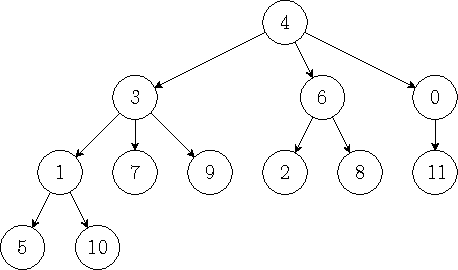
\includegraphics[width=8cm]{images/tree.pdf}
\end{figure}

Tu deber es recorrer el árbol y mostrarlo por niveles, es decir, primero la raiz (nodo 4), luego sus hijos (nodos 3, 6, y 0), después los hijos de estos nodos que se encuentran en el siguiente nivel (nodos 1, 7, 9, 2, 8, y 11), y as\'i sucesivamente. Para el ejemplo de la figura anterior, la respuesta que se busca ser\'ia la siguiente:

\begin{verbatim}
      4
      3 6 0
      1 7 9 2 8 11
      5 10
\end{verbatim}

Pero dependiendo de como se arme el árbol se pueden tener varias respuestas válidas. Para nuestro ejemplo, otra respuesta válida puede ser:

\begin{verbatim}
      4
      6 0 3
      2 8 11 7 9 1 
      10 5
\end{verbatim}

Un \'arbol $ T = (V, E)$ está conformado por un conjunto de v\'ertices $V = \lbrace 0, 2, \dots, n-1\rbrace$, y un conjunto de aristas $E = \lbrace (p, q) / p, q \in V \rbrace$ con la condici\'on de que existe un nodo ra\'iz $r \in V$, y que hay $n-1$ aristas. Cada elemento $(p, q) \in E$, indicar\'a que existe arista desde el nodo $p$ hacia el nodo $q$. Para el ejemplo de la figura anterior, $V = \lbrace 0, 1, 2, 3, 4, 5, 6, 7, 8, 9, 10, 11 \rbrace$, $E=\lbrace(4,3), (4, 6), (4, 0), (3, 1), (3, 7), (3, 9), (6, 2), (6, 8), (0, 11), (1, 5), (1, 10)\rbrace$, el nodo $4$ es el nodo raíz y el árbol tiene $4$ niveles.


\InputFile

La entrada del problema contiene varios casos de prueba. La primera línea es un entero $T$ $(1 \leq T \leq 100)$ indicando el número de casos de prueba. Para cada caso, se sigue el siguiente formato de entrada:

\begin{itemize}
\item La primera línea contiene un entero $N$ indicando la cantidad de nodos del árbol ($1 \leq N \leq 10^3$).

\item La segunda línea contiene $N - 1$ pares de enteros $p, q$ representando las aristas del árbol ($0 \leq p, q < N, p\neq q$). Por claridad, un par de enteros $p, q$ expresa una arista del nodo $p$ hacia el nodo $q$.

\end{itemize}

\OutputFile
Para cada caso de prueba, el programa deber\'a imprimir ``\texttt{Caso \#i:}'' (sin comillas) y a partir de la siguiente linea el árbol por niveles. Como pueden haber varios recorridos por niveles válidos para un mismo árbol, imprimir cualquier recorrido válido.

\Example

\begin{example}
\exmp{%%INPUT
3
2
0 1
5
0 1 1 2 2 3 3 4
12
4 3 3 1 6 2 0 11 3 9 4 0 1 5 6 8 1 10 3 7 4 6%%END-INPUT
}{ %%OUTPUT
Caso \#1:
0
1
Caso \#2:
0
1
2
3
4
Caso \#3:
4
3 6 0
1 7 9 2 8 11
5 10
} %%END-OUTPUT
\end{example}

\end{problem}
